\documentclass[11pt]{article}
\usepackage[margin=0.9in]{geometry}\usepackage{graphicx,booktabs,amsmath,float}
\title{Image-Space Residual INR: Pixel-Supervision Sweep across Change Extent}
\author{Patient-Specific Residual INR --- SLAM Ax\_T2\_2D, change\_extent $\in\{0,1,2\}$}
\date{\today}\begin{document}\maketitle
\section*{Setup}
Image-space reconstruction $\hat{x}=f^{\mathrm{prior}}_\theta+r_\phi$ with the prior INR frozen. The residual is trained on a random fraction $p$ of the follow-up pixels and evaluated on the full image. For each change level the slice with the largest anatomical change is shown. Baselines: \textbf{prior-copy} (DICOM prior) and \textbf{prior-finetune} (NeRP-style: prior INR fine-tuned on the observed follow-up pixels). PBS $\approx1$ preserves change; PBS $\ll1$ suppresses it.
\section*{Frozen prior INR vs.\ DICOM}
How faithfully the prior INR $f^{\mathrm{prior}}_\theta$ reproduces the registered DICOM prior it is frozen from:
\begin{table}[H]\centering\begin{tabular}{lr}\toprule
change\_extent & prior INR PSNR (dB) \\ \midrule
0 & 44.92 \\
1 & 45.59 \\
2 & 44.57 \\
\bottomrule\end{tabular}\end{table}
\begin{figure}[H]\centering
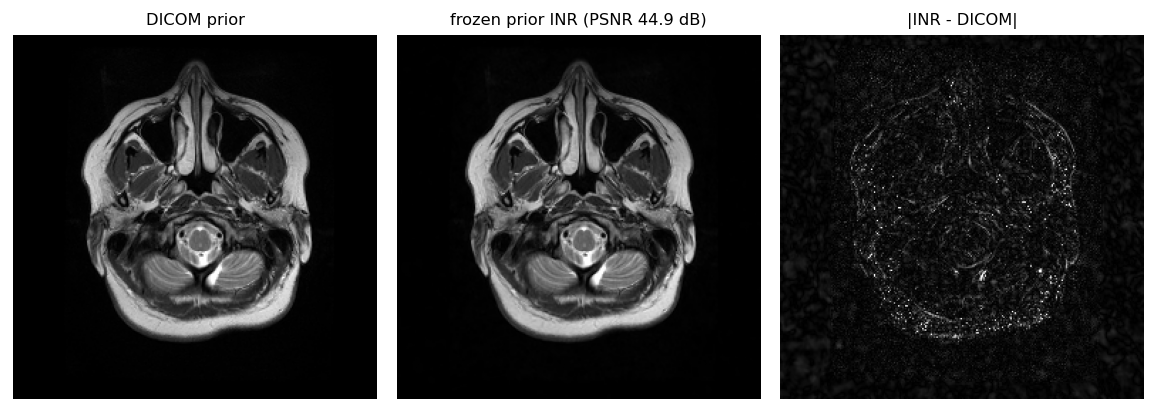
\includegraphics[width=0.8\linewidth]{prior_c0.png}
\caption{change\_extent=0: DICOM prior, the frozen prior INR reconstruction (PSNR 44.9 dB), and their difference.}
\end{figure}
\begin{figure}[H]\centering
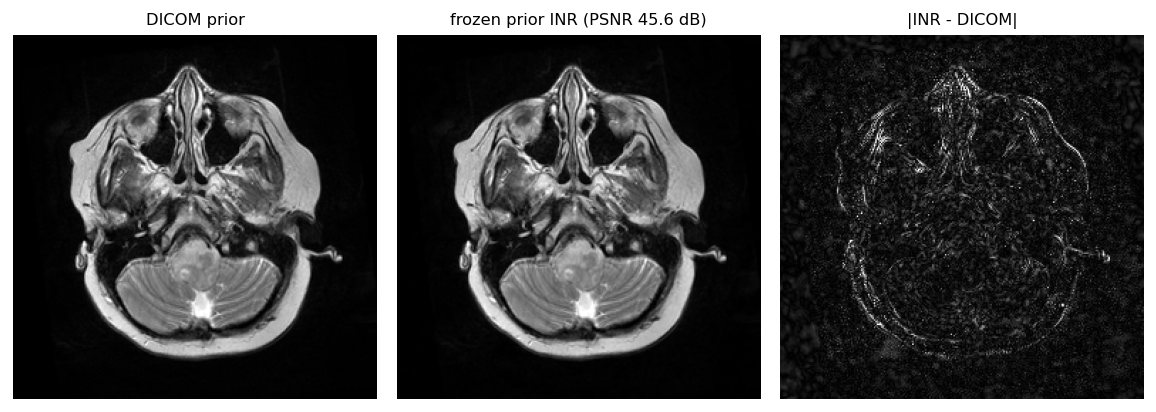
\includegraphics[width=0.8\linewidth]{prior_c1.png}
\caption{change\_extent=1: DICOM prior, the frozen prior INR reconstruction (PSNR 45.6 dB), and their difference.}
\end{figure}
\begin{figure}[H]\centering
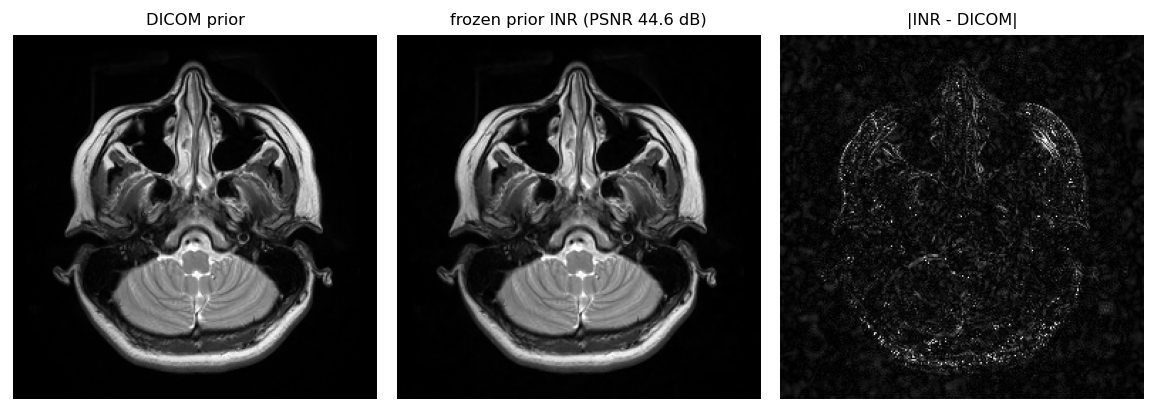
\includegraphics[width=0.8\linewidth]{prior_c2.png}
\caption{change\_extent=2: DICOM prior, the frozen prior INR reconstruction (PSNR 44.6 dB), and their difference.}
\end{figure}
\begin{table}[H]\centering
\caption{Comparison across change extent at $p=50\%$ observed follow-up pixels.}
\begin{tabular}{llrrrrr}\toprule
change & method & PSNR & SSIM & NMSE & CPE & PBS \\ \midrule
0 & prior-copy & 19.45 & 0.677 & 0.1652 & 0.0480 & 0.000 \\
 & prior-finetune (NeRP) & 29.30 & 0.925 & 0.0171 & 0.0132 & 0.978 \\
 & \textbf{prior+residual (ours)} & 26.78 & 0.803 & 0.0306 & 0.0204 & 0.917 \\
\midrule
1 & prior-copy & 15.20 & 0.451 & 0.6423 & 0.0928 & 0.000 \\
 & prior-finetune (NeRP) & 31.88 & 0.923 & 0.0138 & 0.0104 & 0.995 \\
 & \textbf{prior+residual (ours)} & 28.47 & 0.774 & 0.0303 & 0.0186 & 0.954 \\
\midrule
2 & prior-copy & 17.44 & 0.660 & 0.3099 & 0.0705 & 0.000 \\
 & prior-finetune (NeRP) & 30.26 & 0.925 & 0.0162 & 0.0124 & 0.992 \\
 & \textbf{prior+residual (ours)} & 27.78 & 0.807 & 0.0287 & 0.0194 & 0.947 \\

\bottomrule\end{tabular}\end{table}
\begin{table}[H]\centering
\caption{Comparison across change extent at $p=100\%$ observed follow-up pixels.}
\begin{tabular}{llrrrrr}\toprule
change & method & PSNR & SSIM & NMSE & CPE & PBS \\ \midrule
0 & prior-copy & 19.45 & 0.677 & 0.1652 & 0.0480 & 0.000 \\
 & prior-finetune (NeRP) & 47.73 & 0.982 & 0.0002 & 0.0027 & 1.004 \\
 & \textbf{prior+residual (ours)} & 33.87 & 0.875 & 0.0060 & 0.0114 & 0.978 \\
\midrule
1 & prior-copy & 15.20 & 0.451 & 0.6423 & 0.0928 & 0.000 \\
 & prior-finetune (NeRP) & 47.00 & 0.986 & 0.0004 & 0.0025 & 0.996 \\
 & \textbf{prior+residual (ours)} & 34.50 & 0.854 & 0.0076 & 0.0114 & 0.974 \\
\midrule
2 & prior-copy & 17.44 & 0.660 & 0.3099 & 0.0705 & 0.000 \\
 & prior-finetune (NeRP) & 45.55 & 0.985 & 0.0005 & 0.0030 & 0.996 \\
 & \textbf{prior+residual (ours)} & 34.01 & 0.891 & 0.0068 & 0.0112 & 0.978 \\

\bottomrule\end{tabular}\end{table}
\subsection*{change\_extent = 0: full supervision sweep}
\begin{table}[H]\centering\begin{tabular}{llrrrrr}\toprule
$p$ & method & PSNR & SSIM & NMSE & CPE & PBS \\ \midrule
25\% & prior-copy & 19.45 & 0.677 & 0.1652 & 0.0480 & 0.000 \\
 & prior-finetune (NeRP) & 26.20 & 0.869 & 0.0349 & 0.0212 & 0.949 \\
 & \textbf{prior+residual (ours)} & 24.20 & 0.691 & 0.0554 & 0.0289 & 0.871 \\
\midrule
50\% & prior-copy & 19.45 & 0.677 & 0.1652 & 0.0480 & 0.000 \\
 & prior-finetune (NeRP) & 29.30 & 0.925 & 0.0171 & 0.0132 & 0.978 \\
 & \textbf{prior+residual (ours)} & 26.78 & 0.803 & 0.0306 & 0.0204 & 0.917 \\
\midrule
75\% & prior-copy & 19.45 & 0.677 & 0.1652 & 0.0480 & 0.000 \\
 & prior-finetune (NeRP) & 32.97 & 0.961 & 0.0073 & 0.0073 & 0.994 \\
 & \textbf{prior+residual (ours)} & 29.93 & 0.834 & 0.0148 & 0.0150 & 0.968 \\
\midrule
100\% & prior-copy & 19.45 & 0.677 & 0.1652 & 0.0480 & 0.000 \\
 & prior-finetune (NeRP) & 47.73 & 0.982 & 0.0002 & 0.0027 & 1.004 \\
 & \textbf{prior+residual (ours)} & 33.87 & 0.875 & 0.0060 & 0.0114 & 0.978 \\

\bottomrule\end{tabular}
\end{table}
\subsection*{change\_extent = 1: full supervision sweep}
\begin{table}[H]\centering\begin{tabular}{llrrrrr}\toprule
$p$ & method & PSNR & SSIM & NMSE & CPE & PBS \\ \midrule
25\% & prior-copy & 15.20 & 0.451 & 0.6423 & 0.0928 & 0.000 \\
 & prior-finetune (NeRP) & 28.70 & 0.857 & 0.0287 & 0.0166 & 0.982 \\
 & \textbf{prior+residual (ours)} & 25.02 & 0.658 & 0.0670 & 0.0277 & 0.913 \\
\midrule
50\% & prior-copy & 15.20 & 0.451 & 0.6423 & 0.0928 & 0.000 \\
 & prior-finetune (NeRP) & 31.88 & 0.923 & 0.0138 & 0.0104 & 0.995 \\
 & \textbf{prior+residual (ours)} & 28.47 & 0.774 & 0.0303 & 0.0186 & 0.954 \\
\midrule
75\% & prior-copy & 15.20 & 0.451 & 0.6423 & 0.0928 & 0.000 \\
 & prior-finetune (NeRP) & 35.46 & 0.958 & 0.0061 & 0.0061 & 0.995 \\
 & \textbf{prior+residual (ours)} & 31.44 & 0.828 & 0.0153 & 0.0140 & 0.960 \\
\midrule
100\% & prior-copy & 15.20 & 0.451 & 0.6423 & 0.0928 & 0.000 \\
 & prior-finetune (NeRP) & 47.00 & 0.986 & 0.0004 & 0.0025 & 0.996 \\
 & \textbf{prior+residual (ours)} & 34.50 & 0.854 & 0.0076 & 0.0114 & 0.974 \\

\bottomrule\end{tabular}
\end{table}
\subsection*{change\_extent = 2: full supervision sweep}
\begin{table}[H]\centering\begin{tabular}{llrrrrr}\toprule
$p$ & method & PSNR & SSIM & NMSE & CPE & PBS \\ \midrule
25\% & prior-copy & 17.44 & 0.660 & 0.3099 & 0.0705 & 0.000 \\
 & prior-finetune (NeRP) & 27.23 & 0.866 & 0.0325 & 0.0198 & 0.994 \\
 & \textbf{prior+residual (ours)} & 24.99 & 0.761 & 0.0545 & 0.0267 & 0.906 \\
\midrule
50\% & prior-copy & 17.44 & 0.660 & 0.3099 & 0.0705 & 0.000 \\
 & prior-finetune (NeRP) & 30.26 & 0.925 & 0.0162 & 0.0124 & 0.992 \\
 & \textbf{prior+residual (ours)} & 27.78 & 0.807 & 0.0287 & 0.0194 & 0.947 \\
\midrule
75\% & prior-copy & 17.44 & 0.660 & 0.3099 & 0.0705 & 0.000 \\
 & prior-finetune (NeRP) & 34.02 & 0.959 & 0.0068 & 0.0072 & 0.994 \\
 & \textbf{prior+residual (ours)} & 30.47 & 0.862 & 0.0154 & 0.0146 & 0.964 \\
\midrule
100\% & prior-copy & 17.44 & 0.660 & 0.3099 & 0.0705 & 0.000 \\
 & prior-finetune (NeRP) & 45.55 & 0.985 & 0.0005 & 0.0030 & 0.996 \\
 & \textbf{prior+residual (ours)} & 34.01 & 0.891 & 0.0068 & 0.0112 & 0.978 \\

\bottomrule\end{tabular}
\end{table}
\subsection*{Learned residual vs.\ true change (ours)}
\begin{table}[H]\centering\begin{tabular}{lrrrrrr}\toprule
 & \multicolumn{2}{c}{change 0} & \multicolumn{2}{c}{change 1} & \multicolumn{2}{c}{change 2} \\
$p$ & corr & rel-L1 & corr & rel-L1 & corr & rel-L1 \\ \midrule
25\% & 0.810 & 0.620 & 0.926 & 0.318 & 0.894 & 0.399 \\
50\% & 0.898 & 0.445 & 0.967 & 0.214 & 0.946 & 0.293 \\
75\% & 0.952 & 0.333 & 0.984 & 0.161 & 0.971 & 0.221 \\
100\% & 0.980 & 0.255 & 0.992 & 0.133 & 0.987 & 0.172 \\
\bottomrule\end{tabular}\end{table}
\section*{Qualitative panels and residual training convergence (ours)}
\begin{figure}[H]\centering
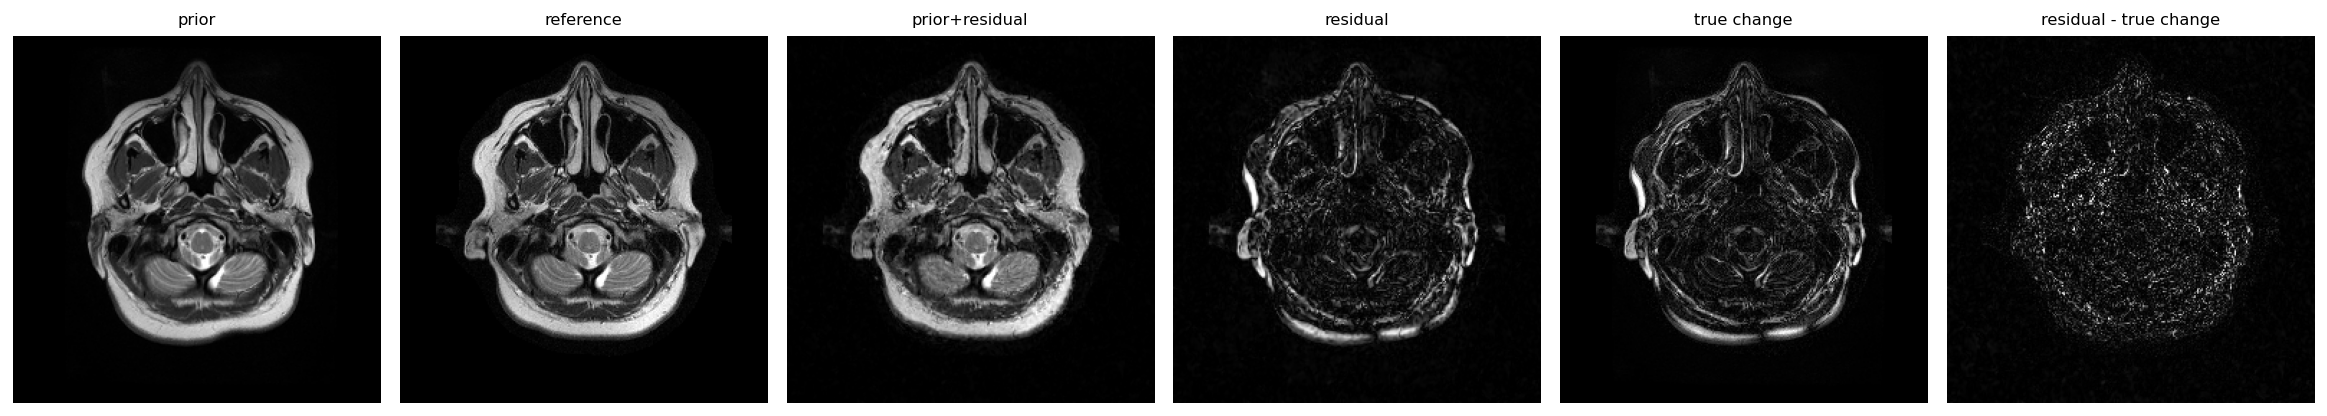
\includegraphics[width=\linewidth]{panel_c0_p050.png}
\caption{change\_extent=0, $p=50\%$. Left to right: prior, reference, prior+residual (ours), learned residual, true change, $|$residual $-$ true change$|$.}
\end{figure}
\begin{figure}[H]\centering
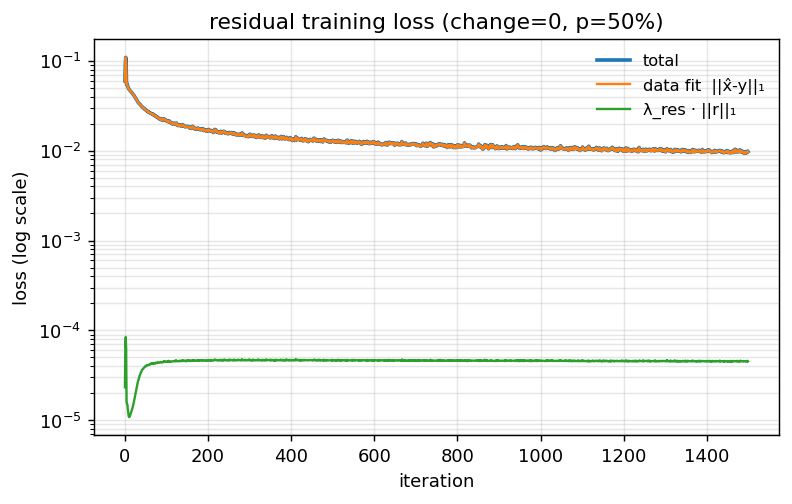
\includegraphics[width=0.62\linewidth]{loss_c0_p050.png}
\caption{Residual training loss (change\_extent=0, $p=50\%$): total and its components (data fit, $\lambda_{\mathrm{res}}\|r\|_1$) on a log axis.}
\end{figure}
\begin{figure}[H]\centering
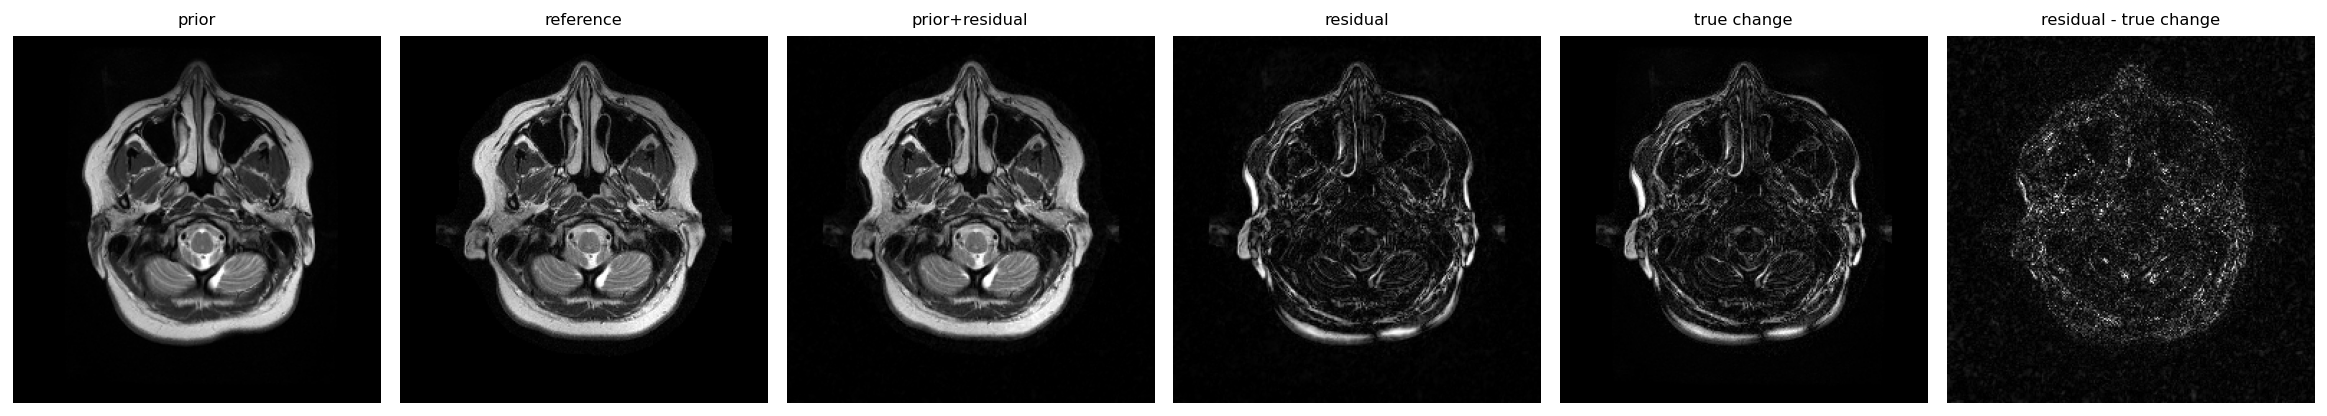
\includegraphics[width=\linewidth]{panel_c0_p100.png}
\caption{change\_extent=0, $p=100\%$. Left to right: prior, reference, prior+residual (ours), learned residual, true change, $|$residual $-$ true change$|$.}
\end{figure}
\begin{figure}[H]\centering
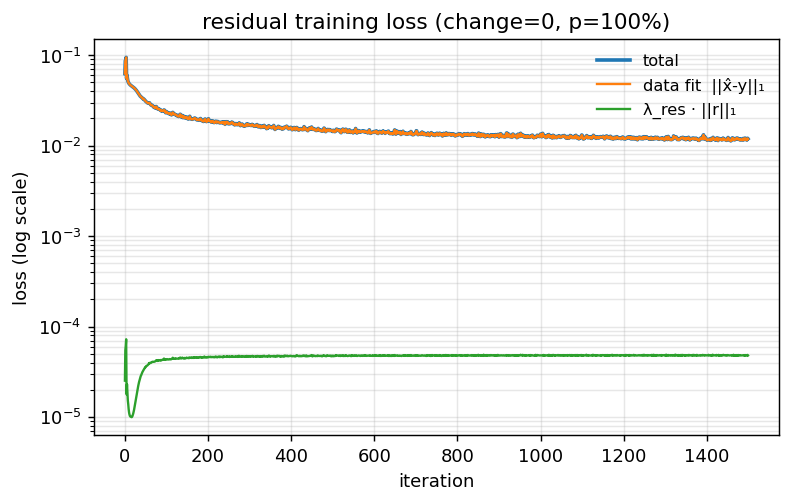
\includegraphics[width=0.62\linewidth]{loss_c0_p100.png}
\caption{Residual training loss (change\_extent=0, $p=100\%$): total and its components (data fit, $\lambda_{\mathrm{res}}\|r\|_1$) on a log axis.}
\end{figure}
\begin{figure}[H]\centering
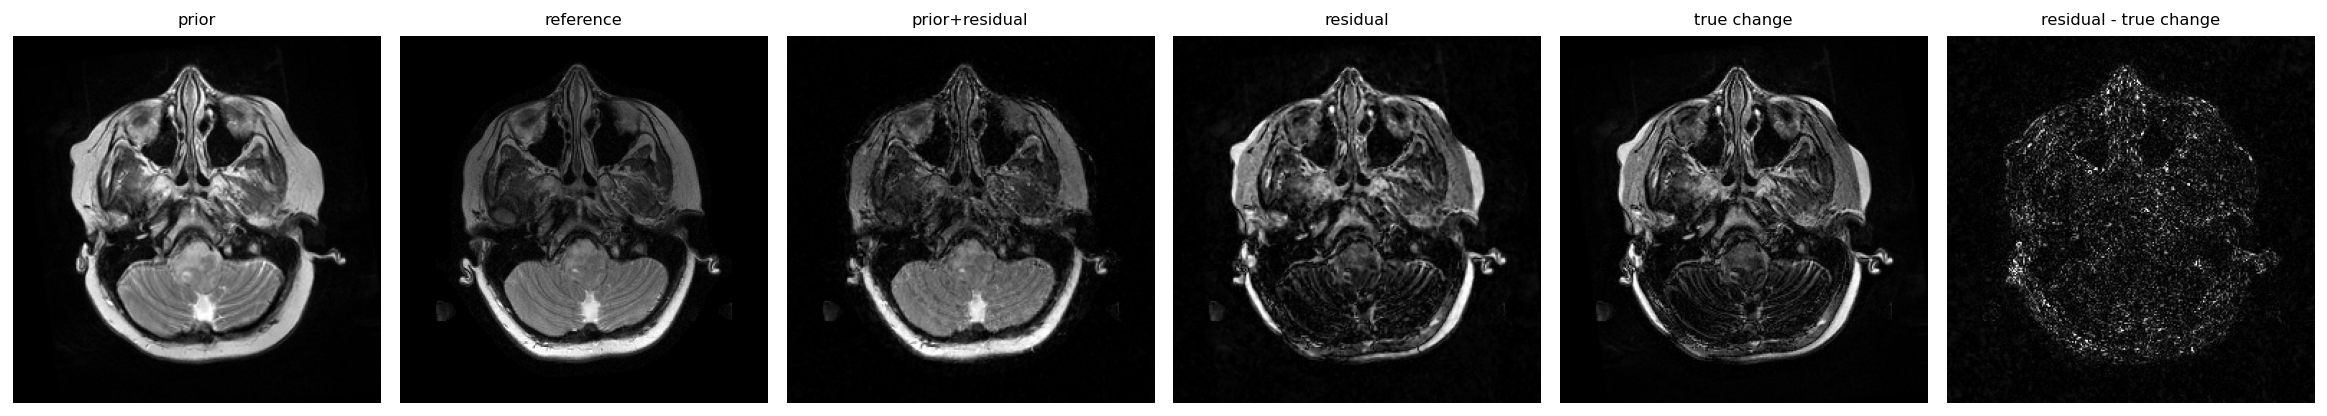
\includegraphics[width=\linewidth]{panel_c1_p050.png}
\caption{change\_extent=1, $p=50\%$. Left to right: prior, reference, prior+residual (ours), learned residual, true change, $|$residual $-$ true change$|$.}
\end{figure}
\begin{figure}[H]\centering
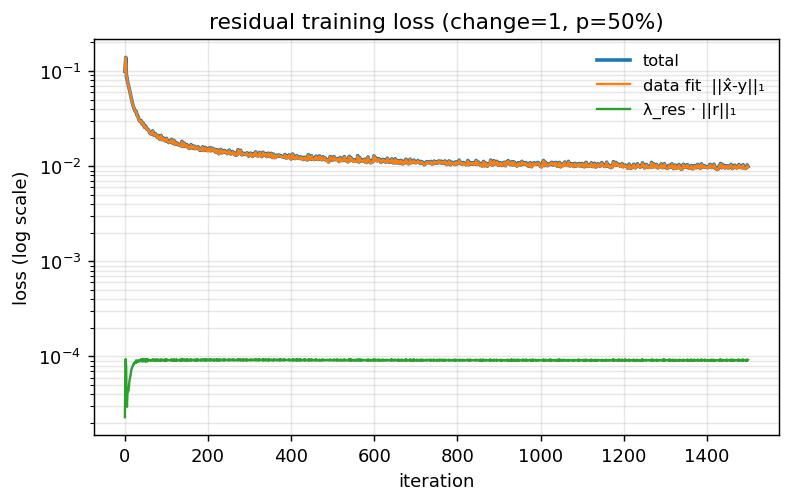
\includegraphics[width=0.62\linewidth]{loss_c1_p050.png}
\caption{Residual training loss (change\_extent=1, $p=50\%$): total and its components (data fit, $\lambda_{\mathrm{res}}\|r\|_1$) on a log axis.}
\end{figure}
\begin{figure}[H]\centering
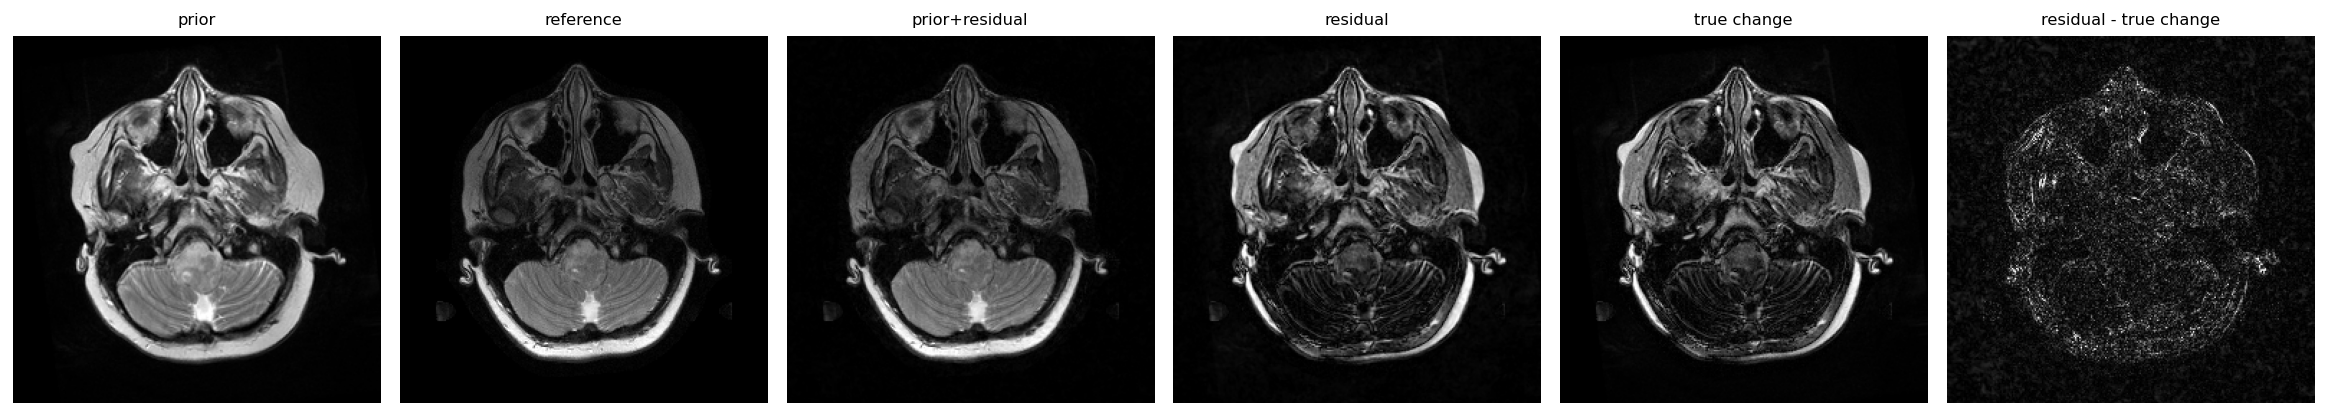
\includegraphics[width=\linewidth]{panel_c1_p100.png}
\caption{change\_extent=1, $p=100\%$. Left to right: prior, reference, prior+residual (ours), learned residual, true change, $|$residual $-$ true change$|$.}
\end{figure}
\begin{figure}[H]\centering
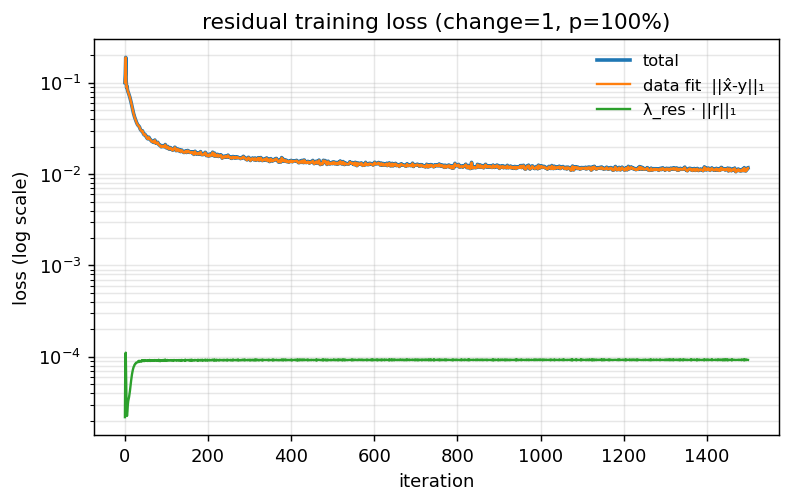
\includegraphics[width=0.62\linewidth]{loss_c1_p100.png}
\caption{Residual training loss (change\_extent=1, $p=100\%$): total and its components (data fit, $\lambda_{\mathrm{res}}\|r\|_1$) on a log axis.}
\end{figure}
\begin{figure}[H]\centering
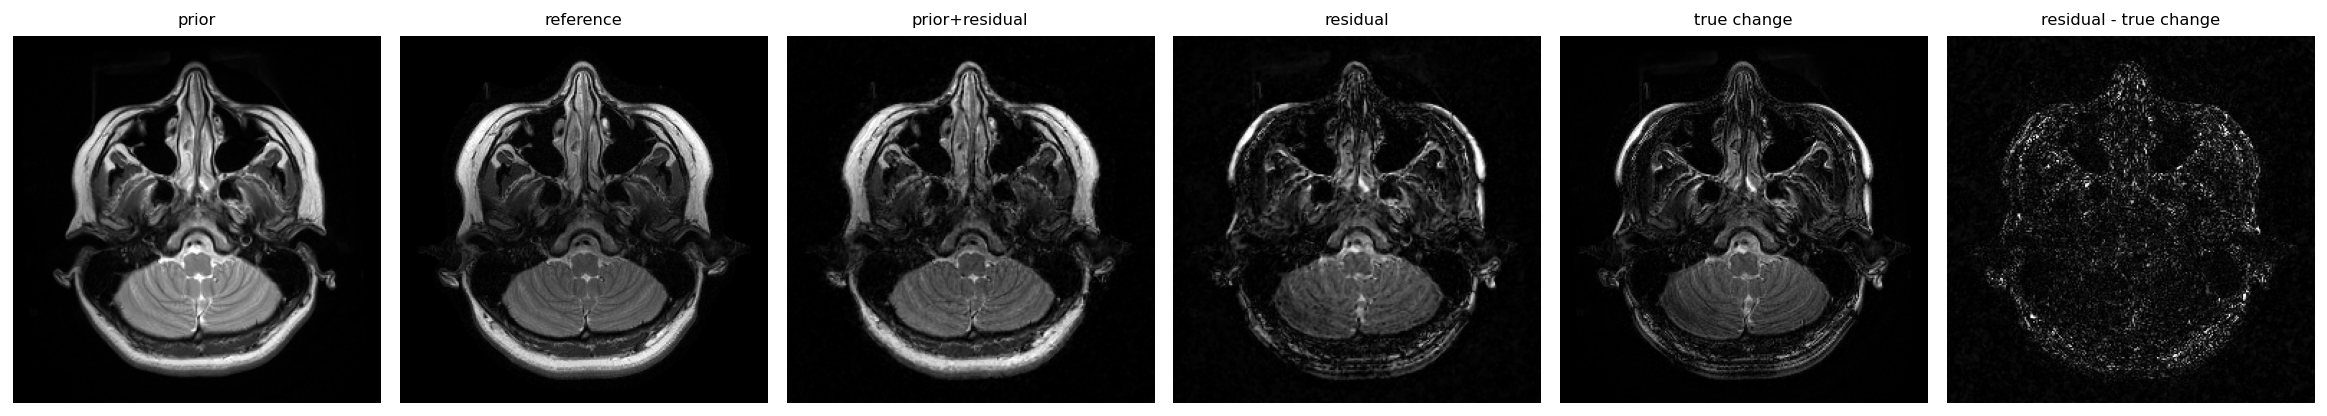
\includegraphics[width=\linewidth]{panel_c2_p050.png}
\caption{change\_extent=2, $p=50\%$. Left to right: prior, reference, prior+residual (ours), learned residual, true change, $|$residual $-$ true change$|$.}
\end{figure}
\begin{figure}[H]\centering
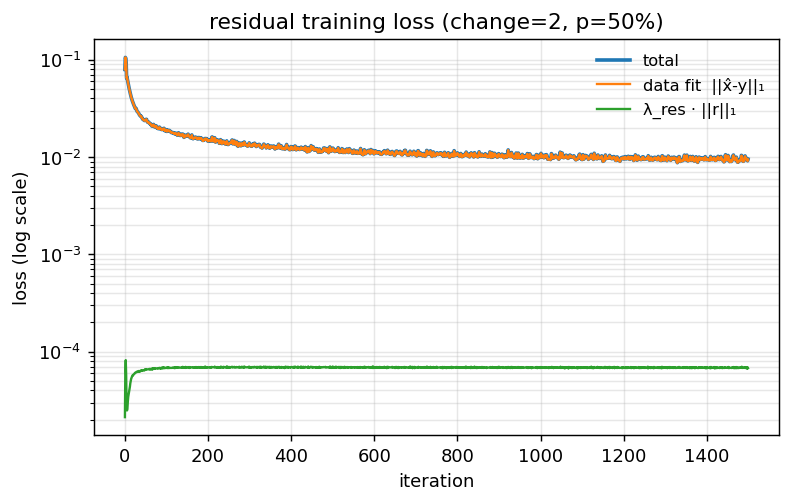
\includegraphics[width=0.62\linewidth]{loss_c2_p050.png}
\caption{Residual training loss (change\_extent=2, $p=50\%$): total and its components (data fit, $\lambda_{\mathrm{res}}\|r\|_1$) on a log axis.}
\end{figure}
\begin{figure}[H]\centering
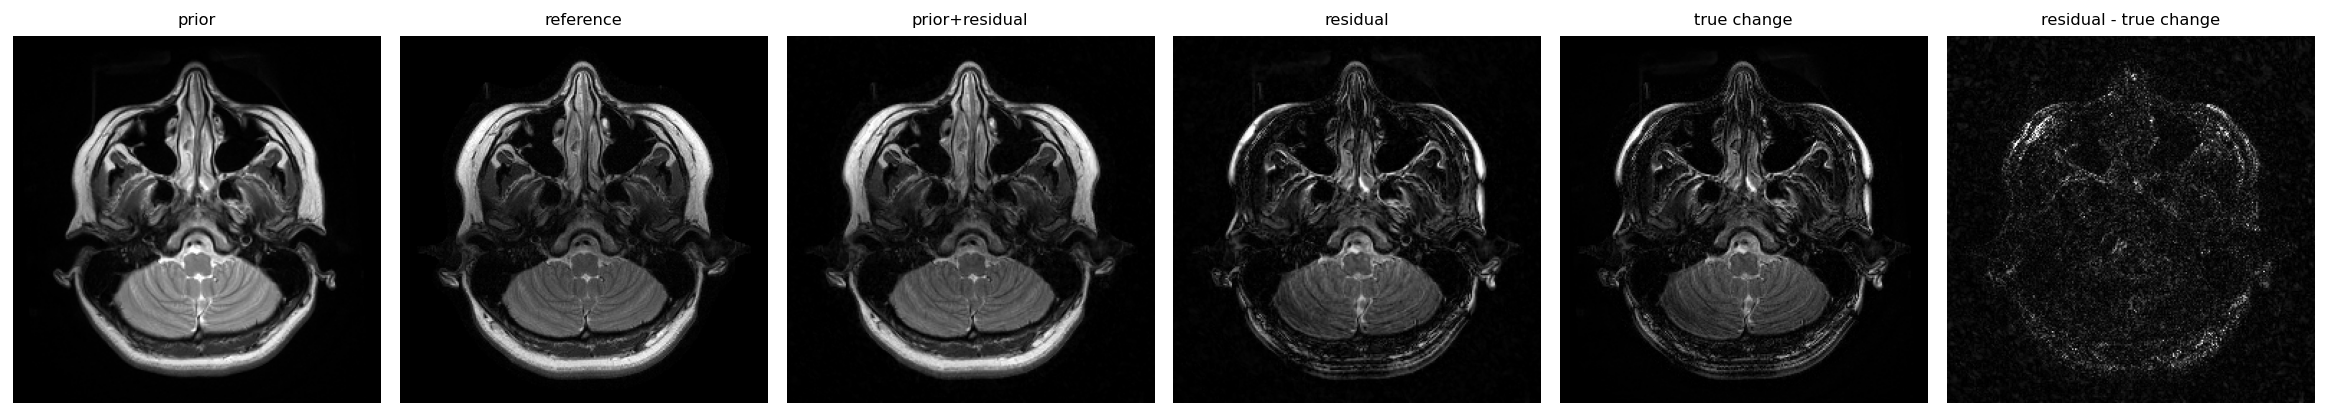
\includegraphics[width=\linewidth]{panel_c2_p100.png}
\caption{change\_extent=2, $p=100\%$. Left to right: prior, reference, prior+residual (ours), learned residual, true change, $|$residual $-$ true change$|$.}
\end{figure}
\begin{figure}[H]\centering
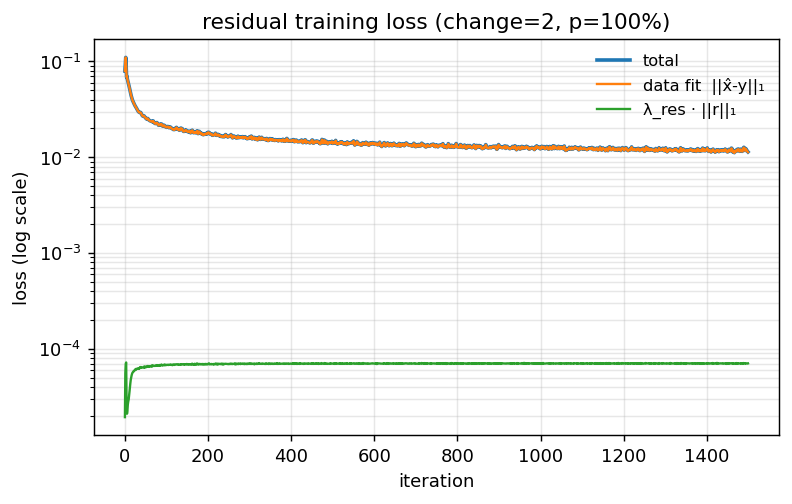
\includegraphics[width=0.62\linewidth]{loss_c2_p100.png}
\caption{Residual training loss (change\_extent=2, $p=100\%$): total and its components (data fit, $\lambda_{\mathrm{res}}\|r\|_1$) on a log axis.}
\end{figure}
\end{document}